\documentclass[12pt,a4paper]{report}
\usepackage{listings}
\usepackage{xcolor} 
%\usepackage{indentfirst}
\usepackage{float}
\usepackage[utf8]{inputenc}
\usepackage[T1]{fontenc}
\usepackage[brazil]{babel}
\usepackage{graphicx}
\usepackage{amsmath, amssymb}
\usepackage{hyperref}
\usepackage{caption}
\captionsetup{labelformat=empty}
\usepackage[a4paper,margin=2.5cm]{geometry}

\setlength{\parindent}{1cm}
\setlength{\parskip}{0.5em}
\lstset{
    inputencoding=utf8,
    extendedchars=true,
    literate={á}{{\'a}}1 {ã}{{\~a}}1 {â}{{\^a}}1 {à}{{\`a}}1
             {é}{{\'e}}1 {ê}{{\^e}}1 {í}{{\'i}}1 {ó}{{\'o}}1
             {ô}{{\^o}}1 {õ}{{\~o}}1 {ú}{{\'u}}1 {ç}{{\c{c}}}1
             {Á}{{\'A}}1 {Ã}{{\~A}}1 {Â}{{\^A}}1 {À}{{\`A}}1
             {É}{{\'E}}1 {Ê}{{\^E}}1 {Í}{{\'I}}1 {Ó}{{\'O}}1
             {Ô}{{\^O}}1 {Õ}{{\~O}}1 {Ú}{{\'U}}1 {Ç}{{\c{C}}}1,
    basicstyle=\small,
    numbers=left,
    numberstyle=\tiny\color{gray},
    stepnumber=1,
    breaklines=true,
    frame=single,
    captionpos=b,
    keywordstyle=\color{blue},
    commentstyle=\color{gray},
    stringstyle=\color{orange}
}
\makeatletter
\renewcommand{\@makechapterhead}[1]{%
  \vspace*{5pt} 
  {\parindent \z@
    \normalfont\Large\bfseries #1\par\nobreak
    \vskip 15pt 
  }}
\makeatother
\setcounter{secnumdepth}{0}

\begin{document}
\frenchspacing

\begin{titlepage}
\begin{figure}[h!] 
    \centering
    
\includegraphics[width=0.2\textwidth]{logo.png}
    \label{fig:logo}
\end{figure}
\begin{center}
    \large
    \textbf{FACULDADE CESAR SCHOOL}\\
    CURSO DE GRADUAÇÃO EM CIÊNCIA DA COMPUTAÇÃO

    \vfill

    \Huge
    \textbf{Análise de Complexidade do Algoritmo de Dijkstra}

    \vfill

    \large
    \textbf{Henrique Magalhães\\
    Júlia Sales\\
    Roberto Catunda}

    \vfill

    \normalsize
    Recife \\
    Junho/2025
\end{center}
\end{titlepage}

\newpage
\tableofcontents
\newpage

\renewcommand{\chaptername}{}  
\renewcommand{\thechapter}{}   

\chapter{1. Introdução}

Este projeto, realizado para a cadeira de Teoria da Computação visa analisar e estudar o algoritmo de Dijkstra, que é responsável por encontrar o caminho mínimo em grafos ponderados com pesos não-negativos. O objetivo é fornecer uma análise teórica de sua complexidade, implementação em duas linguagens (C e Python) e fornecer a análise obtida por meio das simulações feitas.

Links úteis:

- \href{https://colab.research.google.com/drive/12GPpVhj-tCwuHSAhOKFfujmenyjhA5-J?usp=sharing}{Collab utilizado para gerar os gráficos}

- \href{https://github.com/julsales/DijkstraTC}{Github do código fonte}


\chapter{2. Descrição do Algoritmo}

\section*{Conceitos Preliminares}

Antes de descrever o funcionamento do algoritmo de Dijkstra, é importante ressaltar a definição de grafo. Um \textbf{grafo} é uma estrutura matemática usada para modelar relações entre pares de objetos. Ele é composto por um conjunto de \textbf{vértices} (ou \textit{nós}) e um conjunto de \textbf{arestas} (ou \textit{ligações}) que conectam pares desses vértices.

Um grafo pode ser:
\begin{itemize}
  \item \textbf{Não direcionado}: quando as arestas não possuem direção (a ligação é bidirecional);
  \item \textbf{Direcionado}: quando as arestas têm uma direção definida (a ligação vai de um vértice para outro).
\end{itemize}

Além disso, os grafos podem ter \textbf{pesos} associados às arestas. Esses pesos representam custos, distâncias, ou qualquer outra medida relevante ao contexto do problema. Quando cada aresta possui um peso, dizemos que o grafo é \textbf{ponderado}.

\section*{Problema Resolvido}
O problema de Dijkstra propõe que "dado um grafo ponderado e um vértice de origem, deve-se encontrar os caminhos de menor custo da origem a todos os outros vértices, desde que os pesos sejam não-negativos".

\section*{Lógica Geral}
\begin{enumerate}
    \item Inicializar distâncias com infinito, exceto a origem que recebe 0.
    \item Utilizar uma fila de prioridade (min-heap) para explorar vértices com menor custo.
    \item Atualizar distâncias dos vizinhos se um caminho mais curto for encontrado.
    \item Repetir até que todos os vértices tenham sido visitados.
\end{enumerate}

\newpage
\section*{Pseudocódigo}
\begin{lstlisting}[language=Python, caption=Pseudocódigo do algoritmo de Dijkstra]
function Dijkstra(Grafo, origem):
    para cada vértice v:
        dist[v] = infinito
    dist[origem] = 0
    fila = fila de prioridade com (0, origem)

    enquanto fila não vazia:
        (custo, u) = fila.pop()
        para cada vizinho v de u:
            if dist[u] + peso(u,v) < dist[v]:
                dist[v] = dist[u] + peso(u,v)
                fila.insere((dist[v], v))
\end{lstlisting}

\chapter{3. Análise de Complexidade}

\section*{Classificação Assintótica}

Abaixo, é possível ver as complexidades assintóticas do algoritmo de Dijkstra com e sem o uso de heap binário como fila de prioridade.

\subsection*{Versão com heap}
Utiliza uma estrutura de min-heap para otimizar a seleção do menor vértice e atualização das distâncias:

\begin{itemize}
\item \textbf{Melhor caso (Big-Omega $\boldsymbol{\Omega}$):} $\Omega((V + E)\log V)$
\item \textbf{Caso médio (Big-Theta $\boldsymbol{\Theta}$):} $\Theta((V + E)\log V)$
\item \textbf{Pior caso (Big-O $\boldsymbol{O}$):} $O((V + E)\log V)$
\end{itemize}

\subsection*{Versão sem heap}
Utiliza vetor simples como fila de prioridade, com busca linear do menor vértice:

\begin{itemize}
\item \textbf{Melhor caso (Big-Omega $\boldsymbol{\Omega}$):} $\Omega(V^2)$
\item \textbf{Caso médio (Big-Theta $\boldsymbol{\Theta}$):} $\Theta(V^2)$
\item \textbf{Pior caso (Big-O $\boldsymbol{O}$):} $O(V^2)$
\end{itemize}

Embora a versão com heap seja assintoticamente mais eficiente, especialmente em grafos esparsos (quando $E \ll V^2$), a versão utilizada neste projeto, por simplicidade e fins didáticos, foi a \textbf{versão sem heap}.

\chapter{4. Aplicabilidade Prática}

\section*{Eficiência}
Dijkstra é eficiente em:
\begin{itemize}
    \item Grafos esparsos com implementações otimizadas;
    \item Aplicações como GPS, redes de computadores, roteamento e análise de mapas.
\end{itemize}

\section*{Limitações}
\begin{itemize}
    \item Não funciona com pesos negativos;
    \item Pode ser ineficiente em grafos densos sem otimizações.
\end{itemize}

\chapter{5. Simulações e Experimentos}

\section*{Metodologia}
Foram gerados grafos sintéticos com 500, 2500 e 5000 vértices. Cada configuração foi executada 30 vezes. Coletaram-se médias e desvios-padrão dos tempos.

\section*{Ambiente}
\begin{itemize}
    \item Python com \texttt{heapq}, \texttt{time}, \texttt{math} e \texttt{re} (expressões regulares), temporização via \texttt{time.time()}
    \item C com \texttt{stdlib.h}, \texttt{string.h}, \texttt{limits.h}, \texttt{time.h} e \texttt{clock()}
\end{itemize}

\section*{Resultados}
Após a simulação foram obtidos os seguintes tempos de execução:
\begin{lstlisting}[language=Python, caption= Tempos de Execução, basicstyle=\tiny]
tempo_c_500v = [0.001000, 0.001000, 0.001000, 0.001000, 0.001000, 0.001000, 0.001000, 0.001000, 0.002000, 0.001000,
                0.002000, 0.000000, 0.002000, 0.001000, 0.000000, 0.002000, 0.000000, 0.001000, 0.001000, 0.001000,
                0.002000, 0.001000, 0.001000, 0.000000, 0.002000, 0.001000, 0.001000, 0.001000, 0.000000, 0.002000
                ]
tempo_c_2500v = [0.033000, 0.031000, 0.025000, 0.032000, 0.033000, 0.030000, 0.019000, 0.031000, 0.028000, 0.016000,
                 0.033000, 0.025000, 0.025000, 0.033000, 0.022000, 0.029000, 0.014000, 0.026000, 0.030000, 0.026000,
                 0.027000, 0.033000, 0.034000, 0.032000, 0.024000, 0.024000, 0.026000, 0.028000, 0.023000, 0.025000
                 ]
tempo_c_5000v = [0.079000, 0.079000, 0.081000, 0.074000, 0.074000, 0.145000, 0.066000, 0.065000, 0.075000, 0.066000,
                 0.081000, 0.074000, 0.077000, 0.074000, 0.075000, 0.073000, 0.081000, 0.072000, 0.073000, 0.079000,
                 0.070000, 0.091000, 0.072000, 0.072000, 0.075000, 0.075000, 0.074000, 0.074000, 0.074000, 0.063000
                ]

tempo_py_500v = [0.016766, 0.011546, 0.017674, 0.013368, 0.009649, 0.012738, 0.010895, 0.004226, 0.007728, 0.011580,
                 0.007661, 0.001975, 0.016578, 0.014068, 0.012457, 0.011945, 0.007076, 0.010749, 0.019350, 0.006499,
                 0.007542, 0.012465, 0.010211, 0.013160, 0.012552, 0.003705, 0.017359, 0.015390, 0.014620, 0.014852
                ]
tempo_py_2500v = [0.257263, 0.153051, 0.184478, 0.319510, 0.276850, 0.124794, 0.035414, 0.288510, 0.164211, 0.273675,
                  0.298736, 0.210732, 0.278545, 0.313726, 0.315531, 0.199445, 0.320459, 0.100062, 0.104913, 0.064756,
                  0.308222, 0.106224, 0.051615, 0.243700, 0.184594, 0.405185, 0.310464, 0.159756, 0.023914, 0.154531
                 ]
tempo_py_5000v = [0.560904, 1.228559, 1.233382, 0.827072, 2.104762, 1.627338, 1.357748, 0.199732, 0.274592, 0.999782,
                  0.468814, 0.249466, 0.505003, 1.056147, 1.041142, 0.450411, 1.102306, 1.448330, 1.794473, 1.456239,
                  1.448483, 0.356798, 0.131758, 1.783411, 0.608467, 1.223389, 0.084121, 1.133065, 1.112486, 0.192759
                 ]
\end{lstlisting}

\newpage

\textbf{Dados coletados em Python:}
\begin{itemize}
    \item \textbf{500 vértices}:
    \begin{itemize}
        \item Média: 0{,}011546 segundos
        \item Desvio-padrão: 0{,}004246
    \end{itemize}
    \item \textbf{2500 vértices}:
    \begin{itemize}
        \item Média: 0{,}207762 segundos
        \item Desvio-padrão: 0{,}099867
    \end{itemize}
    \item \textbf{5000 vértices}:
    \begin{itemize}
        \item Média: 0{,}935365 segundos
        \item Desvio-padrão: 0{,}555800
    \end{itemize}
\end{itemize}

\vspace{0.5em}
\textbf{Dados coletados em C:}
\begin{itemize}
    \item \textbf{500 vértices}:
    \begin{itemize}
        \item Média: 0{,}001067 segundos
        \item Desvio-padrão: 0{,}000629
    \end{itemize}
    \item \textbf{2500 vértices}:
    \begin{itemize}
        \item Média: 0{,}027233 segundos
        \item Desvio-padrão: 0{,}005051
    \end{itemize}
    \item \textbf{5000 vértices}:
    \begin{itemize}
        \item Média: 0{,}076767 segundos
        \item Desvio-padrão: 0{,}013778
    \end{itemize}
\end{itemize}

\section*{Gráficos Obtidos}
\begin{figure}[H]
    \centering
    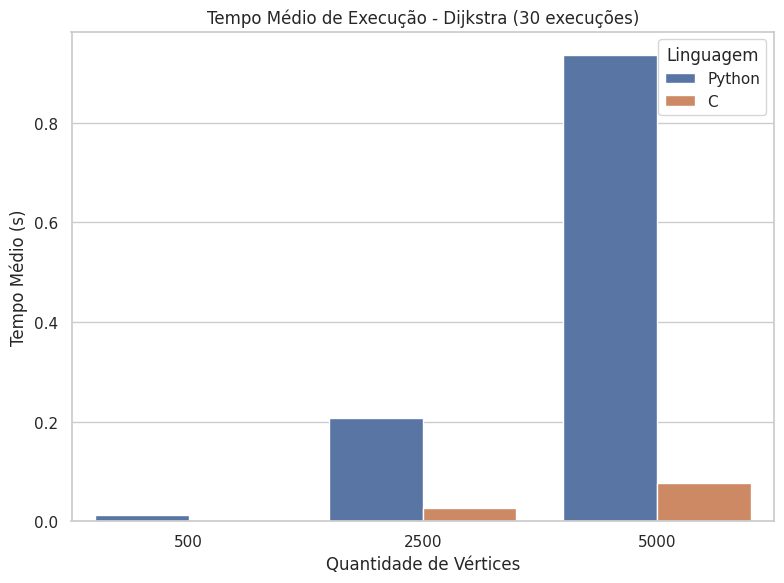
\includegraphics[width=1\textwidth]{tempo_medio.png}
    \caption{Comparação de tempos médios (C vs. Python)}
\end{figure}

\begin{figure}[H]
    \centering
    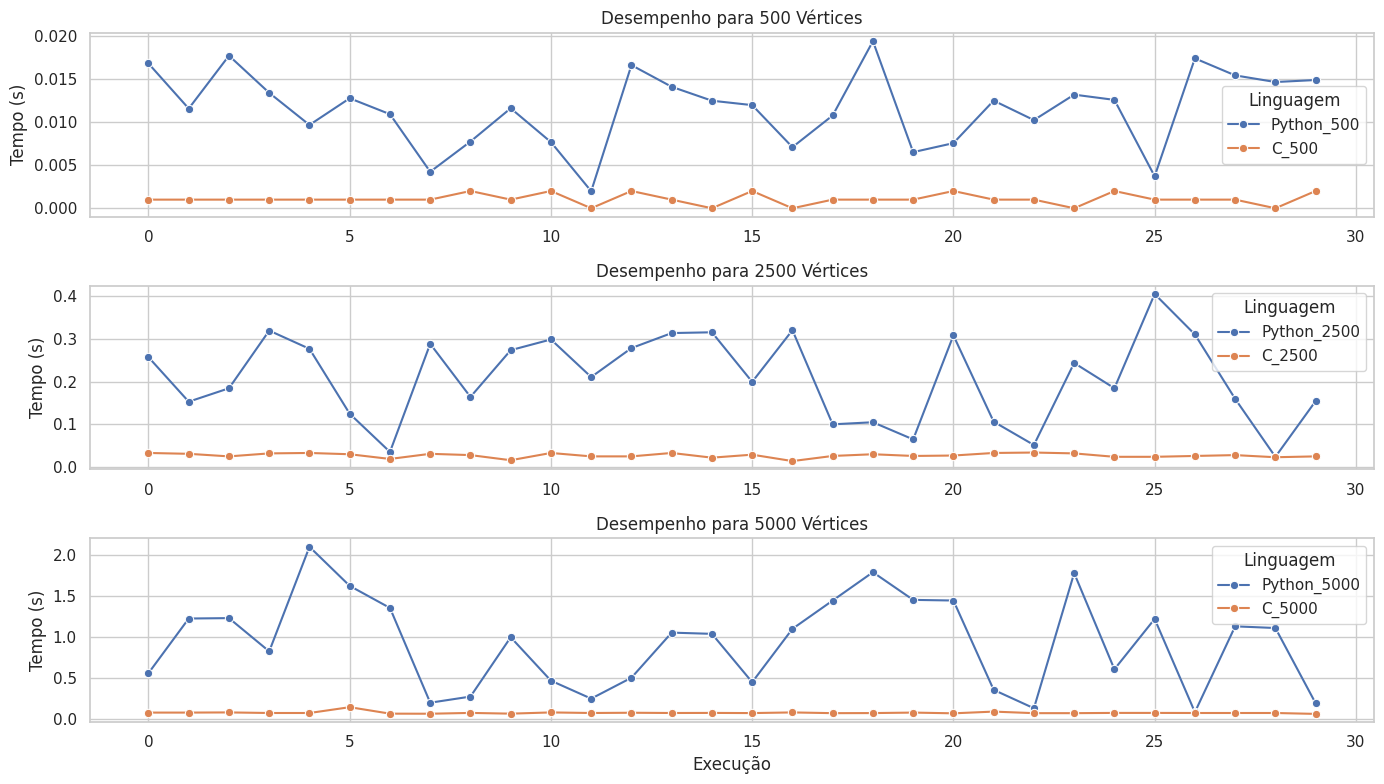
\includegraphics[width=1\textwidth]{desempenho.png}
    \caption{(Comparação do desempenho por quantidade de vértices (C vs. Python)}
\end{figure}

\chapter{6. Análise de Casos}
\begin{itemize}
    \item \textbf{Melhor caso (Big-Omega $\boldsymbol{\Omega}$):} Mesmo no melhor caso, o \texttt{min()} linear precisa varrer $V$ elementos em cada iteração, resultando em $\Omega(V^2)$.
    
    \item \textbf{Caso médio (Big-Theta $\boldsymbol{\Theta}$):} A cada iteração, é feita uma busca linear pelo vértice de menor custo, seguida da atualização dos vizinhos. O comportamento médio permanece $\Theta(V^2)$.
    
    \item \textbf{Pior caso (Big-O $\boldsymbol{O}$):} Em um grafo denso, todas as arestas são relaxadas e cada busca pelo menor custo percorre $V$ vértices, totalizando $O(V^2)$.
\end{itemize}
\section*{Conclusões}
Mesmo no melhor caso, o algoritmo de Dijkstra sem heap precisa realizar uma busca linear para encontrar o vértice de menor custo ainda não visitado. Isso significa que, independentemente da estrutura do grafo, cada iteração envolve uma varredura completa dos vértices, resultando em complexidade $\Omega(V^2)$. No caso médio, o algoritmo percorre a lista de vértices para selecionar o próximo vértice a ser processado e atualiza seus vizinhos, mantendo o mesmo comportamento em $\Theta(V^2)$. No pior cenário, como em grafos densos, todas as arestas são examinadas, e o vértice de menor distância é procurado a cada iteração, totalizando um custo de $O(V^2)$.


\chapter{7. Código-Fonte}

\section*{7.1 Implementação em C}
\begin{lstlisting}[language=C, caption=Dijkstra em C (parcial)]
#include <stdio.h>
#include <stdlib.h>
#include <string.h>
#include <limits.h>
#include <time.h>

#define MAX_VERTICES 6000  // Aumentado para suportar vértices grandes
#define INF INT_MAX

typedef struct {
    int destino;
    int peso;
} Aresta;

Aresta grafo[MAX_VERTICES][MAX_VERTICES];
int grau[MAX_VERTICES] = {0};
int numVertices = 0;

int nomeParaIndice(const char *nome) {
    return atoi(nome);  // Sem prefixo "v"
}

void adicionarAresta(const char *origemStr, int peso, const char *destinoStr) {
    int origem = nomeParaIndice(origemStr);
    int destino = nomeParaIndice(destinoStr);

    if (origem >= 0 && destino >= 0) {
        grafo[origem][grau[origem]].destino = destino;
        grafo[origem][grau[origem]].peso = peso;
        grau[origem]++;

        grafo[destino][grau[destino]].destino = origem;
        grafo[destino][grau[destino]].peso = peso;
        grau[destino]++;

        if (origem >= numVertices) numVertices = origem + 1;
        if (destino >= numVertices) numVertices = destino + 1;
    }
}

// Leitura robusta para arquivos com uma linha gigante
void lerArquivo(const char *nomeArquivo) {
    FILE *file = fopen(nomeArquivo, "r");
    if (!file) {
        perror("Erro ao abrir arquivo");
        exit(1);
    }

    char token[200];
    int pos = 0;

    char origem[20], destino[20];
    int peso;

    int ch;
    while ((ch = fgetc(file)) != EOF) {
        if (ch == '|') {
            token[pos] = '\0';
            if (sscanf(token, "%[^-(]-(%d)-%[^ \n]", origem, &peso, destino) == 3) {
                adicionarAresta(origem, peso, destino);
            }
            pos = 0;
        } else {
            if (pos < sizeof(token) - 1) {
                token[pos++] = ch;
            }
        }
    }

    // Último token (caso não termine com '|')
    if (pos > 0) {
        token[pos] = '\0';
        if (sscanf(token, "%[^-(]-(%d)-%[^ \n]", origem, &peso, destino) == 3) {
            adicionarAresta(origem, peso, destino);
        }
    }

    fclose(file);
}

void dijkstra(int origem, int destino) {
    int distancia[MAX_VERTICES], visitado[MAX_VERTICES] = {0}, anterior[MAX_VERTICES];
    for (int i = 0; i < MAX_VERTICES; i++) {
        distancia[i] = INF;
        anterior[i] = -1;
    }

    distancia[origem] = 0;

    clock_t inicio = clock();

    for (int i = 0; i < numVertices; i++) {
        int u = -1;
        for (int j = 0; j < numVertices; j++) {
            if (!visitado[j] && (u == -1 || distancia[j] < distancia[u])) {
                u = j;
            }
        }

        if (u == -1 || distancia[u] == INF) break;

        visitado[u] = 1;

        for (int k = 0; k < grau[u]; k++) {
            int v = grafo[u][k].destino;
            int peso = grafo[u][k].peso;

            if (distancia[u] + peso < distancia[v]) {
                distancia[v] = distancia[u] + peso;
                anterior[v] = u;
            }
        }
    }

    clock_t fim = clock();
    double tempo_execucao = (double)(fim - inicio) / CLOCKS_PER_SEC;

    if (distancia[destino] == INF) {
        printf("Não há caminho entre %d e %d.\n", origem, destino);
        return;
    }

    int caminho[MAX_VERTICES];
    int tamanho = 0, atual = destino;

    while (atual != -1) {
        caminho[tamanho++] = atual;
        atual = anterior[atual];
    }

    printf("Menor caminho: ");
    for (int i = tamanho - 1; i >= 0; i--) {
        printf("%d", caminho[i]);
        if (i > 0) printf(" -> ");
    }

    printf("\nCusto total: %d\n", distancia[destino]);
    printf("Tempo de execução: %.6f segundos\n", tempo_execucao);
}
//grafo_multigrafo_500_pipe
//grafo_multigrafo_2500_pipe
//grafo_multigrafo_5000_pipe
int main() {
    char nomeArquivo[] = "grafo_multigrafo_5000_pipe.txt";
    lerArquivo(nomeArquivo);
    printf("Grafo carregado com %d vértices.\n", numVertices);

    char origemStr[20], destinoStr[20];
    int origem, destino;

    printf("Digite o vértice de origem (ex: 0): ");
    scanf("%s", origemStr);
    printf("Digite o vértice de destino (ex: 500): ");
    scanf("%s", destinoStr);

    origem = nomeParaIndice(origemStr);
    destino = nomeParaIndice(destinoStr);

    if (origem < 0 || destino < 0 || origem >= MAX_VERTICES || destino >= MAX_VERTICES) {
        printf("Vértices inválidos.\n");
        return 1;
    }

    dijkstra(origem, destino);

    return 0;
}
\end{lstlisting}

\section*{7.2 Implementação em Python}
\begin{lstlisting}[language=Python, caption=Dijkstra em Python (parcial)]
import tkinter as tk
from tkinter import messagebox, scrolledtext
import re
import time
import math

# Variáveis globais para deslocamento do grafo (pan)
offset_x = 0
offset_y = 0
_last_mouse_x = None
_last_mouse_y = None

# === Lógica do Dijkstra ===
def parse_input(data):
    graph = {}
    edges = data.strip().split('|')

    for edge in edges:
        match = re.match(r'([A-Za-z0-9]+)-\(([\d.]+)\)-([A-Za-z0-9]+)', edge.strip())
        if not match:
            raise ValueError(f"Formato inválido na aresta: '{edge}'")

        v1, peso, v2 = match.groups()
        peso = float(peso)

        if v1 not in graph:
            graph[v1] = []
        if v2 not in graph:
            graph[v2] = []

        graph[v1].append((v2, peso))
        graph[v2].append((v1, peso))  # Remova se for direcionado

    return graph

def dijkstra_path(graph, start, end):
    distances = {node: float('inf') for node in graph}
    previous = {node: None for node in graph}
    distances[start] = 0
    visited = set()
    queue = list(graph.keys())

    while queue:
        # Buscar o nó com menor distância (substitui heapq.heappop)
        current_node = min((node for node in queue if node not in visited), key=lambda node: distances[node], default=None)
        if current_node is None:
            break
        queue.remove(current_node)
        visited.add(current_node)

        if current_node == end:
            break

        for neighbor, weight in graph[current_node]:
            if neighbor in visited:
                continue
            distance = distances[current_node] + weight
            if distance < distances[neighbor]:
                distances[neighbor] = distance
                previous[neighbor] = current_node

    # Reconstruir caminho
    path = []
    cur = end
    if distances[end] == float('inf'):
        return float('inf'), []
    while cur is not None:
        path.append(cur)
        cur = previous[cur]
    path.reverse()

    return distances[end], path


# === Função para desenhar grafo no canvas com caminho destacado ===
def desenhar_grafo(canvas, graph, caminho=None):
    global offset_x, offset_y
    canvas.delete("all")
    if not graph:
        return

    largura = int(canvas['width'])
    altura = int(canvas['height'])
    raio_no = 20

    nodes = list(graph.keys())
    n = len(nodes)
    cx, cy = largura // 2 + offset_x, altura // 2 + offset_y
    raio_circulo = min(largura//2, altura//2) - 50
    pos = {}

    for i, node in enumerate(nodes):
        ang = 2 * math.pi * i / n
        x = cx + int(raio_circulo * math.cos(ang))
        y = cy + int(raio_circulo * math.sin(ang))
        pos[node] = (x, y)

    # Criar conjunto das arestas do caminho para destacar
    arestas_caminho = set()
    if caminho and len(caminho) > 1:
        for i in range(len(caminho) - 1):
            a, b = caminho[i], caminho[i+1]
            arestas_caminho.add((a, b))
            arestas_caminho.add((b, a))  # Para facilitar comparação (grafo não-direcionado)

    # Desenhar arestas
    desenhadas = set()
    for v1, vizinhos in graph.items():
        for v2, peso in vizinhos:
            if (v2, v1) in desenhadas:
                continue
            x1, y1 = pos[v1]
            x2, y2 = pos[v2]
            if caminho and (v1, v2) in arestas_caminho:
                cor = 'red'
                largura_linha = 3
            else:
                cor = 'gray'
                largura_linha = 1
            canvas.create_line(x1, y1, x2, y2, fill=cor, width=largura_linha)
            xm, ym = (x1+x2)//2, (y1+y2)//2
            canvas.create_text(xm, ym, text=str(peso), fill='blue', font=('Arial', 10, 'bold'))
            desenhadas.add((v1, v2))

    # Desenhar nós
    for node, (x, y) in pos.items():
        if caminho and node in caminho:
            fill = 'lightcoral'
            outline = 'red'
            largura_borda = 3
        else:
            fill = 'lightyellow'
            outline = 'black'
            largura_borda = 1
        canvas.create_oval(x - raio_no, y - raio_no, x + raio_no, y + raio_no, fill=fill, outline=outline, width=largura_borda)
        canvas.create_text(x, y, text=node, font=('Arial', 12, 'bold'))

# === Eventos para arrastar o canvas (pan) ===
def iniciar_arrasto(event):
    global _last_mouse_x, _last_mouse_y
    _last_mouse_x = event.x
    _last_mouse_y = event.y

def arrastar(event):
    global offset_x, offset_y, _last_mouse_x, _last_mouse_y, grafo
    dx = event.x - _last_mouse_x
    dy = event.y - _last_mouse_y
    offset_x += dx
    offset_y += dy
    _last_mouse_x = event.x
    _last_mouse_y = event.y
    # Redesenhar com o novo offset
    if grafo:
        desenhar_grafo(canvas_grafo, grafo)
    else:
        canvas_grafo.delete("all")

# === Interface Tkinter ===
def adicionar_grafo():
    global grafo, offset_x, offset_y
    entrada = texto_grafo.get("1.0", tk.END).strip()
    if not entrada:
        messagebox.showwarning("Aviso", "Digite o grafo antes de adicionar.")
        return
    try:
        start_time = time.time()
        grafo = parse_input(entrada)
        # Resetar offset ao carregar novo grafo
        offset_x = 0
        offset_y = 0
        end_time = time.time()
        messagebox.showinfo("Sucesso", f"Grafo adicionado com sucesso!\nTempo de processamento: {(end_time - start_time):.4f}s")
        desenhar_grafo(canvas_grafo, grafo)
    except Exception as e:
        messagebox.showerror("Erro", str(e))

def executar_dijkstra():
    global grafo
    if grafo is None:
        messagebox.showwarning("Aviso", "Adicione o grafo antes de executar o Dijkstra.")
        return

    origem = entrada_origem.get().strip()
    destino = entrada_destino.get().strip()

    if not origem or not destino:
        messagebox.showwarning("Aviso", "Informe o vértice de origem e o de destino.")
        return
    if origem not in grafo or destino not in grafo:
        messagebox.showerror("Erro", "Origem ou destino não estão presentes no grafo.")
        return

    start_time = time.time()
    custo, caminho = dijkstra_path(grafo, origem, destino)
    end_time = time.time()

    texto_resultado.delete("1.0", tk.END)
    if custo == float('inf'):
        texto_resultado.insert(tk.END, f"Não existe caminho entre {origem} e {destino}.\n")
        desenhar_grafo(canvas_grafo, grafo)  # Mostrar grafo completo, pois não há caminho
    else:
        texto_resultado.insert(tk.END, f"Caminho mais curto entre {origem} e {destino}:\n")
        texto_resultado.insert(tk.END, " → ".join(caminho) + "\n")
        texto_resultado.insert(tk.END, f"Custo total: {custo}\n")
        texto_resultado.insert(tk.END, f"Tempo de execução: {(end_time - start_time):.6f} segundos\n")

        # Construir subgrafo com só os nós do caminho e arestas entre eles (consecutivas)
        subgrafo = {}
        for node in caminho:
            subgrafo[node] = []

        for i in range(len(caminho) - 1):
            v1 = caminho[i]
            v2 = caminho[i + 1]
            # Achar peso da aresta no grafo original
            peso = None
            for vizinho, p in grafo[v1]:
                if vizinho == v2:
                    peso = p
                    break
            if peso is None:
                peso = 0  # fallback

            subgrafo[v1].append((v2, peso))
            subgrafo[v2].append((v1, peso))  # Grafo não-direcionado

        desenhar_grafo(canvas_grafo, subgrafo, caminho)

def mostrar_grafo_completo():
    global offset_x, offset_y
    if grafo:
        # Resetar offset ao mostrar grafo completo
        offset_x = 0
        offset_y = 0
        desenhar_grafo(canvas_grafo, grafo)
    else:
        messagebox.showwarning("Aviso", "Nenhum grafo carregado para mostrar.")

# Variável global para armazenar o grafo
grafo = None

# === Janela principal ===
janela = tk.Tk()
janela.title("Dijkstra com Visualização do Grafo")
janela.geometry("1440x800")

# --- Frame esquerda: Entrada, controles e resultado em baixo ---
frame_esquerda = tk.Frame(janela, width=500)
frame_esquerda.pack(side=tk.LEFT, fill=tk.Y, padx=10, pady=10)

# Frame para entrada e controles no topo do lado esquerdo
frame_controles = tk.Frame(frame_esquerda)
frame_controles.pack(side=tk.TOP, fill=tk.X)

tk.Label(frame_controles, text="Digite o grafo (v1-(peso)-v2 separados por '|'):", justify=tk.LEFT).pack(anchor=tk.W)
texto_grafo = scrolledtext.ScrolledText(frame_controles, height=15, wrap=tk.NONE, width=80)
texto_grafo.pack(pady=5)

btn_adicionar = tk.Button(frame_controles, text="Adicionar Grafo", command=adicionar_grafo)
btn_adicionar.pack(pady=5)

frame_vertices = tk.Frame(frame_controles)
frame_vertices.pack(pady=10, fill=tk.X)

tk.Label(frame_vertices, text="Vértice Origem:").grid(row=0, column=0, sticky=tk.W)
entrada_origem = tk.Entry(frame_vertices, width=10)
entrada_origem.grid(row=0, column=1, padx=5)

tk.Label(frame_vertices, text="Vértice Destino:").grid(row=1, column=0, sticky=tk.W)
entrada_destino = tk.Entry(frame_vertices, width=10)
entrada_destino.grid(row=1, column=1, padx=5)

btn_calcular = tk.Button(frame_controles, text="Calcular Menor Caminho", command=executar_dijkstra)
btn_calcular.pack(pady=10)

btn_mostrar_completo = tk.Button(frame_controles, text="Mostrar Grafo Completo", command=mostrar_grafo_completo)
btn_mostrar_completo.pack(pady=5)

# Frame para o resultado embaixo, dentro da esquerda
frame_resultado = tk.Frame(frame_esquerda)
frame_resultado.pack(side=tk.BOTTOM, fill=tk.BOTH, expand=True, pady=(10,0))

tk.Label(frame_resultado, text="Resultado:").pack(anchor=tk.W)
texto_resultado = scrolledtext.ScrolledText(frame_resultado, height=10, wrap=tk.WORD)
texto_resultado.pack(fill=tk.BOTH, expand=True)

# --- Frame direita: canvas ocupando tudo ---
frame_direita = tk.Frame(janela)
frame_direita.pack(side=tk.RIGHT, fill=tk.BOTH, expand=True, padx=10, pady=10)

canvas_grafo = tk.Canvas(frame_direita, width=700, height=900, bg='white', highlightthickness=1, highlightbackground='black')
canvas_grafo.pack(fill=tk.BOTH, expand=True)

# Bind dos eventos para arrastar
canvas_grafo.bind("<ButtonPress-1>", iniciar_arrasto)
canvas_grafo.bind("<B1-Motion>", arrastar)

# Iniciar loop principal
janela.mainloop()

\end{lstlisting}

\chapter{8. Reflexão Final}

O algoritmo de Dijkstra pertence à classe P, pois é resolvido em tempo polinomial. Embora ele não se relacione diretamente com a classe NP, algumas variações do problema, como encontrar caminhos mínimos com restrições (por exemplo, número limitado de vértices ou custo total limitado), podem levar a problemas NP-completos. Além disso, o Dijkstra serve como base para algoritmos mais sofisticados, como o A*, amplamente utilizado em otimização de rotas e inteligência artificial. Seu papel é essencial no desenvolvimento de soluções para problemas combinatórios onde o custo de transição entre estados é um fator relevante.

\end{document}
%-----------------------------
% REFERÊNCIAS
%-----------------------------
%\newpage
%\addcontentsline{toc}{chapter}{9. Referências}
%\begin{thebibliography}{99}
    %\bibitem{ref1} SOBRENOME, Nome. \textit{Título do livro ou artigo}. Editora, ano.
    %\bibitem{ref2} OUTRO AUTOR. \textit{Outro título}. Local: Editora, ano.
%\end{thebibliography}
